%\documentclass[10pt]{article}
\documentclass{sigplanconf}
\usepackage{times,url}
\usepackage{code} 
%\usepackage{proof}
%\usepackage{newcode}
%\usepackage{epsfig}
\usepackage{psfig}

\newcommand{\cut}[1]{}

\newcommand{\appref}[1]{Appendix~\ref{#1}}
\newcommand{\secref}[1]{Section~\ref{#1}}
\newcommand{\tblref}[1]{Table~\ref{#1}}
\newcommand{\figref}[1]{Figure~\ref{#1}}
\newcommand{\listingref}[1]{Listing~\ref{#1}}
%\newcommand{\pref}[1]{{page~\pageref{#1}}}

\newcommand{\eg}{{\em e.g.}}
\newcommand{\cf}{{\em cf.}}
\newcommand{\ie}{{\em i.e.}}
\newcommand{\etc}{{\em etc.\/}}
\newcommand{\naive}{na\"{\i}ve}
\newcommand{\role}{r\^{o}le}
\newcommand{\forte}{{fort\'{e}\/}}
\newcommand{\appr}{\~{}}

\newcommand{\bftt}[1]{{\ttfamily\bfseries{}#1}}
\newcommand{\kw}[1]{\bftt {#1}}
\newcommand{\Pthen}{\kw{Pthen}}
\newcommand{\pads}{\textsc{pads}}
\newcommand{\padsl}{\textsc{padsl}}
\newcommand{\padst}{\textsc{pads/t}}
\newcommand{\datatype}{\textsc{PADS/T}}
%\newcommand{\datatype}{\textsc{DataType}}
\newcommand{\C}{\textsc{C}}
\newcommand{\perl}{\textsc{Perl}}
\newcommand{\ml}{\textsc{ml}}
\newcommand{\sml}{\textsc{sml}}
\newcommand{\smlnj}{\textsc{sml/nj}}
\newcommand{\java}{\textsc{java}}
\newcommand{\ddl}{\textsc{ddl}}
\newcommand{\xml}{\textsc{xml}}
\newcommand{\datascript}{\textsc{DataScript}}
\newcommand{\packettypes}{\textsc{PacketTypes}}
\newcommand{\erlang}{\textsc{Erlang}}

\newcommand{\Core}{Ad hoc}
\newcommand{\core}{ad hoc}
\newcommand{\pvalue}{\core{} value}
\newcommand{\ppat}{\core{} pattern}
\newcommand{\ptype}{\core{} type}

\newcommand{\padsc}{\textsc{pads}/\C{}}
\newcommand{\padsml}{\textsc{pads}/\ml{}}

\newcommand{\dibbler}{Sirius}
\newcommand{\ningaui}{Altair}
\newcommand{\darkstar}{Regulus}

\newcommand{\pdgood}{{\tt G}}
\newcommand{\pdbad}{{\tt B}}
\newcommand{\pdnest}{{\tt N}}
\newcommand{\pdsem}{{\tt S}}
\newcommand{\ptypes}{T}
\newcommand{\patreadpd}[2]{{\tt #1<<#2>>}}
\newcommand{\btm}{\cd{BOT}}


\newcommand{\lsem}{{[\![}}
\newcommand{\rsem}{{]\!]}}


\newcommand{\figHeight}[4]{\begin{figure}[tb]
	\centerline{
	            \epsfig{file=#1,height=#4}}
	\caption{#2}
	\label{#3}
	\end{figure}}

%% Environment for typesetting BNF grammars. Uses display math mode.
\newenvironment{bnf}
     {%% local command definitions:
        %% BNF definition symbol
      \def\->{\rightarrow}
%%      \def\::={{::=} &}
      \def\::={\bnfdef &}
      \def\|{\bnfalt}
      \newcommand{\name}[1]{\text{##1}}
        %% non-terminal
      \newcommand{\nont}[1]{{##1}}
      \newcommand{\meta}[1]{& ##1 &}
      \newcommand{\descr}[1]{& \text{// ##1}}
      \newcommand{\opt}[1]{ [##1] }
      \newcommand{\opnon}[1]{\opt{\nont{##1}}}
      \newcommand{\none}{\epsilon}
      \newcommand{\nwln}{\\ &&&}
      \newcommand{\nlalt}{\\ && \| &}
      \[\begin{array}{lrlll}
     }
     {\end{array}\]}

\newcommand{\mcd}[1]{\mathtt{#1}}
\newcommand{\ppair}[3]{#1{:}#2 \mathrel{**} #3}
\newcommand{\parray}[3]{#1\;\mcd{Parray}(#2,#3)}
\newcommand{\pset}[3]{\{#1{:}#2\,|\,#3\}}
\newcommand{\pstream}[1]{#1\;\mcd{stream}}
\newcommand{\precord}[1]{\{\{#1\}\}}


% %%%%%%%%%%%%%%%%%%%%%%%%%%%%%%%%%%%%%%%%%%%%%%%%%%%%%%%%%%%%%%%%%%%%%%%%%%%%
% \voffset             0in    %  top vertical offset
% \hoffset             0in    %  left horizontal offset
% \oddsidemargin       0pt    %  Left margin on odd-numbered pages.
% \evensidemargin      0pt    %  Left margin on even-numbered pages.
% \topmargin           0pt    %  Nominal distance from top of page to top of
% \headheight          0pt    %  Height of box containing running head.
% \headsep             0pt    %  Space between running head and text.
% \textwidth         6.5in    %  Width of text on page
% \textheight          9in    %  Height of text on page
% \setlength{\parskip}{.05in}
% \renewcommand{\floatpagefraction}{.9}
% \renewcommand{\textfraction}{0.1}
% % \renewcommand{\baselinestretch}{1.01}
% %\input{macro}  %%%  other macro definitions


\title{Semi-automatic Generation of Systems Monitoring Tools \\ (Work in Progress)}

\authorinfo{Kathleen Fisher \quad Yitzhak Mandelbaum \quad Vivek Pai \quad David Walker
}{AT\&T Research and Princeton University}

%%%%%%%%%%%%%%%%%%%%%%%%%%%%%%%%%%%%%%%%%%%%%%%%%%%%%%%%%%%%%%%%%%%%%%%%%%%%
\begin{document}

\maketitle{}

\begin{abstract}
Complex systems must be {\em monitored} to proactively find problems,
record/archive system health, oversee system operation, detect
malicious processes or security violations and perform a myriad of other 
tasks.  In this work, we propose a new, general-purpose architecture 
for development and maintenance of systems monitors, whether they
be for small-scale single-node processes or wide-area, 
distributed systems.  Our proposal is based on using 
a domain-specific programming language that allows users to specify
properties and requirements of a monitoring system at a high-level
of abstraction.  Given such a high-level specification,
a compiler will automatically generate a collection of
reliable, secure, and high-performance libraries as well as stand-alone
tools that perform all of the basic functions of a monitoring system
including concurrently {\em fetching} data from any number of distributed
sources, {\em archiving} (self-describing) data for later analysis,
{\em querying} data to troubleshoot problems, and {\em displaying}
statistical data summaries so users can monitor system health in real time.
\end{abstract}

\section{Introduction}
\label{sec:intro}

Complex systems must be {\em monitored} to proactively find problems,
record/archive system health, oversee system operation, detect
malicious processes or security violations, and perform a myriad of
other tasks.  The {\em monitoring subsystems} that perform these tasks
take a wide range of forms, from embedded sensors that monitor
physical processes to intrusion detection systems that monitor flows
to a single organization to large-scale systems that monitor the
health and performance of hundreds to thousands of nodes on the Grid.

At the heart of such monitoring systems is a complex, multifaceted
data processing problem that involves, at a minimum, the following
components.
\begin{enumerate}
\item collection and aggregation of information 
distributed across the monitored system.
\item data archiving for later querying, measurement, security auditing and 
post-mortem defect detection
\item querying and information extraction from archived or current, online data
\item presentation and graphical display to administrators and users.
\end{enumerate}

A substantial part of the difficulty of building secure, reliable, efficient,
and evolving monitoring systems is the diversity, quality, and volume of data
these systems must often handle.  Often, new monitoring
systems face the problem of having to interact with legacy devices,
legacy software and legacy data, leaving implementers in a situation
where they cannot use robust off-the-shelf data management tools built for
standard formats like XML.  As a result, implementers simply
hack ``one-off'' monitoring tools of their own, which are invariably
less reliable, unoptimized, insecure, and difficult or impossible to evolve
when new requirements become known.  
We call the nonstandard, disorganized data that monitoring systems
must deal with {\em ad hoc data}.  \figref{figure:data-sources} presents 
a selection of the data used in different monitoring systems, together 
with their size and some of the common problems that arise.


%    These formats, by definition,
% have no standard data processing tools associated with them.
% \figref{figure:data-sources} presents a selection of such formats
% used in a variety of different monitoring systems.
% They include ASCII, binary, and Cobol data formats, with
% both fixed and variable-width records, ranging in size from
% relatively small files through network applications which process over
% a gigabyte per second.  Common errors in the data include undocumented data,
% corrupted data, missing data, and multiple missing-value
% representations.

\begin{figure*}
\begin{center}
\begin{tabular}{|l|l|l|l|l|}
\hline
Name \& Use   &  Representation              &Size           & Sample Problems \\ \hline\hline
Web server logs (CLF): &  Fixed-column  & $\leq$12GB/week & Race conditions \\ 
Measuring web workloads         &  ASCII records &                 & on log entry \\
                                &                &                 & Unexpected values\\ \hline
CoMon data:              &  Geographically & 600 MB/day & Remote failures\\ 
Monitor \& troubleshoot  &  distributed    & collected from           &  \\
PlanetLab infrastructure &  ASCII records  & \appr{}400-450 machines           & \\\hline
AT\&T provisioning data (\dibbler{}): & Variable-width  & 2.2GB/week & Unexpected values \\ 
Monitoring service activation & ASCII records  &            & Corrupted data feeds \\ \hline
Phone call detail:   &  Fixed-width   &\appr{}7GB/day &  Undocumented data\\ 
Fraud detection & binary records & & \\  \hline 
AT\&T billing data (\ningaui{}): & Various Cobol  & \appr{}4000 files/day, & Unexpected values\\ 
Monitoring billing process   & data formats            & 250-300GB/day    & Corrupted data feeds \\ \hline
IP backbone data (\darkstar{})  & ASCII  & $\ge$ 15 sources  & Multiple missing-value \\
Monitoring network performance  &        & \appr{}15 GB/day              & representations  \\ 
                                &        &                               & Undocumented data \\\hline
Netflow       & Data-dependent \# of     & $\ge$1Gigabit/second  & Missed packets\\ 
Monitoring network performance              &  fixed-width    &                       & \\ 
               & binary records & & \\ \hline
\end{tabular}
\caption{Selected ad hoc data sources for system monitoring. }
\label{figure:data-sources}
\end{center}
\end{figure*}

% Processing this sort of 
% ad hoc data is challenging for a variety of other reasons. 
% First, when the data comes from legacy software, sources or devices, it 
% typically just arrives ``as is'': the analysts
% who receive it can only say ``thank you,'' not request a more
% convenient format.  Second, documentation for the format may not exist
% at all, or it may be out of date.  A common phenomenon is for a field
% in a data source to fall into disuse.  After a while, a new piece of
% information becomes interesting, but compatibility issues prevent data
% suppliers from modifying the shape of their data, so instead they
% hijack the unused field, often failing to update the documentation in
% the process.

% Third, such data frequently contain errors, for a variety of reasons:
% malfunctioning equipment, race conditions on log entry~\cite{wpp},
% non-standard values to indicate ``no data available,'' human error in
% entering data, unexpected data values, \etc{} The appropriate response
% to such errors depends on the application.  Some applications require
% the data to be error free: if an error is detected, processing needs
% to stop immediately and a human must be alerted.  Other applications
% can repair the data, while still others can simply discard erroneous
% or unexpected values.  For some applications, errors in the data can
% be the most interesting part because they can signal where two systems
% are failing to communicate.  Monitoring systems may need to respond to such
% errors immediately and effectively.

% Fourth, online monitoring systems
% are highly susceptible to attack from malicious outsiders.
% For example, intrusion detection systems
% and performance evaluation systems that monitor network activity 
% may be sent malicious packets or other data that cause buffer overflows
% and allow attackers to take control of, evade, dismantle or corrupt these
% systems.  A cautionary example of the dangers of online ad hoc data
% processors is the Ethereal system~\cite{ethereal}. Ethereal is used by network administrators for monitoring, analyzing
% and troubleshooting networks. Unfortunately, like most network software, users have found a number of
% vulnerabilities in the software, and moreover many of these vulnerabilities are directly related to the mundane
% components of the system that parse ad hoc data as opposed to the parts of the system that perform
% higher-level tasks. For instance, in March 2004, Stefan Esser posted an advisory on 13 different buffer over-
% flow attacks on Ethereal~\cite{etherealvulnerabilities}. Of the 13, 9 attacks occurred during parsing. These problems are not merely theoretical -- it was
% a buffer overflow in a security monitoring system that was exploited by the
% Witty Worm~\cite{witty}.

% Fifth, ad hoc data sources can be high volume:
% AT\&T's call-detail stream contains roughly 300~million calls per day
% requiring approximately 7GBs of storage space. Although this data is
% eventually archived in a database, analysts mine it profitably before
% such archiving~\cite{kdd98,kdd99}. More challenging, the \ningaui{}
% project at AT\&T accumulates billing data at a rate of 250-300GB/day,
% with occasional spurts of 750GBs/day. Netflow data arrives from Cisco
% routers at rates over a gigabyte per second~\cite{gigascope}! Such
% volumes mean performance is critical and it certainly
% must be possible to process the data without loading
% it all into memory at once.

% Finally, before anything can be done with an ad hoc data source,
% someone has to produce a suitable parser for it.  Today, people tend
% to use \C{} or \perl{} for this task.  Unfortunately, writing parsers
% this way is tedious and error-prone, complicated by the lack of
% documentation, convoluted encodings designed to save space, the need
% to produce efficient code, and the need to handle errors robustly to
% avoid corrupting downstream data.  Moreover, the parser writers'
% hard-won understanding of the data ends up embedded in parsing code,
% making long-term maintenance difficult for the original writers and
% sharing the knowledge with others nearly impossible.

\paragraph*{Specification-driven Monitor Generation.}
This paper describes work-in-progress towards construction
of a new framework for semi-automatic generation of
construction system monitors. In this new framework
we call {\em specification-driven monitor generation}, programmers
describe the shape and properties of data manipulated by
the monitoring system using a domain-specific language and a compiler automatically
generates efficient, reliable, and secure
monitoring tools from that specification.
More specifically, the system will consist of the 
following components:

\begin{enumerate}

\item A high-level specification language to describe a monitor's
data sources.  The specification language will be able to
concisely and accurately describing any ad hoc data source,
including its format, semantic properties, location, and
temporal attributes in an easy-to-understand, easy-to-modify syntax.

\item A compiler that takes data specifications as inputs and
automatically generates a suite of 
efficient data processing libraries for parsing, printing, error detection
and correction, distributed data gathering, compression, and 
reformatting of ad hoc data.

\item A fully automatic tool generator that links the compiler-generated 
libraries to format-independent tool stubs to produce easy-to-use 
tools for high-level tasks including data display and querying.

\end{enumerate}

\begin{figure*}[t]
\begin{center}
\centerline{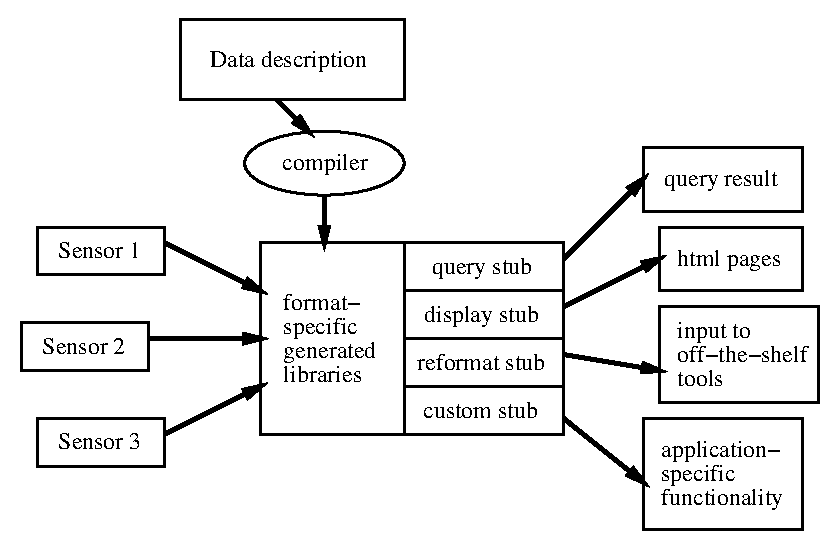
\psfig{file=arch_idraw_edit.ps,height=2.5in}}
\end{center}
\caption{\label{fig:arch} Architecture of Specification-Driven Monitor Generator.
}
\end{figure*}

In the follow section, we will explain 
the general architecture of a specification-driven monitor generation system
in more detail.
Section~\ref{sec:pads} continues by briefly describing PADS, the specification language
we will use as a foundation for our specification-driven monitor generation system.
Section~\ref{sec:framework} focuses on the key systems components that make up the back end of
the specification-driven monitor generation system.  Finally,
Sections~\ref{sec:related} and \ref{sec:conclusion} discuss related work and
conclude.

\section{Specification-Driven Monitor Generation}
\label{sec:architecture}

Figure~\ref{fig:arch} presents the architecture of our proposed
system.  At the top of the picture is the declarative description of all
data that will be used by the monitoring system.  It is here that
programmers encode all their knowledge about their data sources,
including the physical layout of data, its semantic properties
(including constraints on data fields and expected relations
with other fields) so deviations can be flagged as errors, 
its location, access protocol, when the data
will be ready for fetching and how often, etc.

In exchange for the programmer's work in describing their
data sources, the compiler system will generate
a robust and efficient library of {\em format-specific routines} (the center
square in the picture).
The core format-specific 
library includes parser, printer, error detection and data traversal
routines.  The core libraries will also be responsible for controlling
access to and aggregation of any data distributed across wide area
networks and archiving local data along with its description.  

Since these core libraries are compiler-generated from a
high-level data specification, they have many advantages over
hand-written code.  First, the generated code checks
all possible error cases: system errors related to the input file,
buffer, socket, or remote data provider; 
syntax errors related to deviations in the physical
format; and semantic errors in which the data violates user
constraints.  Because these checks appear only in generated code, they
do not clutter the high-level declarative description of the data
source.  Moreover, since tools are generated
automatically by a compiler rather than written by hand, 
they are far more likely to be robust
and far less likely to have dangerous vulnerabilities such as
buffer overflows.  Moreover, as formats change and are updated,
one can make a small change in the high-level description
and the compiler takes care of the rest.  It is extremely unlikely
new vulnerabilities or buffer overflows will be added to the code
base over time as formats change.  Finally, all routines will
be highly optimized for processing the massive
data sets one sees in practice.

In addition to the compiler, which generates the core, format-specific
libraries, the system includes a number of {\em format-independent stubs}
that make use of the generated libraries and implement higher-level
functionality.  Each of these stubs are programmed once, independent
of any format.  In order to implement application-specific behavior, they
are linked with the core libraries, which will be carefully designed to
satisfy a generic, format-independent interface.  Examples of
format-independent tools include a generic query engine that
allows users to extract information from the data, 
a visualization tool that produces
web page summaries of data statistics or a reformatter to convert data
to a new format required by an off-the-shelf tool.  In addition,
a programmer may simply use the generated format-specific libraries directly 
within their own application program, custom built for some unique task. 
Of course whenever a programmer builds a new tool for their application, 
they may do so using the format-independent interface to the generated
libraries.  If they do so, their new tool may be reused by others
who have different data, but require a similar functionality.

At this point, the astute reader may ask why not simply generate
exactly one tool -- a translator that maps the ad hoc data into
XML, a standard format with hundreds of available tools and
rich programming support in all modern, widely used languages.
The problem with such an architecture is that ad hoc formats
are usually quite compact and exploding them into XML representations
can easily result in a space blowup of 8-10 times and an increase
in processing overhead.  Consequently, tiny
sensors in a sensor network cannot afford the expense (processor,
network bandwidth, battery life) of managing
XML data.  More generally, when the data sets get large, and we 
have seen they do in monitoring systems, 
ranging from 100s of MB/week to 100GB/day,
the extra overhead of a 10 times blowup is simply unaffordable.
While compression can reduce this impact, the decompression overheads
of most modern compressors can overwhelm the data processing overhead
of the underlying data.
%In an environment where the data is being used and updated
%by more than just the monitoring system, maintaining a parallel
%representation in XML is even more painful.

\section{PADS:  A Format Description Language}
\label{sec:pads}

PADS~\cite{fisher+:pads,launchpads,fisher+:700,mandelbaum+:padsml} is 
a family of domain-specific languages, and associated compiler technology, 
designed to allow programmers to specify the structure of ad hoc data sources, 
and to generate tools for querying, analyzing and manipulating data in the specified formats.

To understand further how the \pads{} can be used to describe the sorts of data used by system monitors,
let us look at an example of a simple ad hoc data source:
a tiny fragment of data in the Common Log Format (CLF) that web
servers use to log client requests~\cite{wpp}.  
This ASCII format consists of a sequence of
records, each of which has seven fields: the host name or IP address
of the client making the request, the account associated with the
request on the client side, the name the user provided for
authentication, the time of the request, the actual request, the
\textsc{http} response code, and the number of bytes returned as a
result of the request.  The actual request has three parts: the
request method (\eg, \texttt{GET}, \texttt{PUT}), the requested
\textsc{uri}, and the protocol version.  In addition, the second and
third fields are often recorded only as a '-' character to indicate
the server did not record the actual data.  \figref{figure:clf-records}
shows a couple of typical records.

\begin{figure*}
\begin{footnotesize}
%\begin{center}
\begin{verbatim}
207.136.97.49 - - [15/Oct/1997:18:46:51 -0700] "GET /tk/p.txt HTTP/1.0" 200 30
234.200.68.71 - - [15/Oct/1997:18:53:33 -0700] "GET /tr/img/gift.gif HTTP/1.0" 200 409
240.142.174.15 - - [15/Oct/1997:18:39:25 -0700] "GET /tr/img/wool.gif HTTP/1.0" 404 178
188.168.121.58 - - [16/Oct/1997:12:59:35 -0700] "GET / HTTP/1.0" 200 3082
tj62.aol.com - - [16/Oct/1997:14:32:22 -0700] "POST /spt/dd@grp.org/cfm HTTP/1.0" 200 941
214.201.210.19 ekf - [17/Oct/1997:10:08:23 -0700] "GET /img/new.gif HTTP/1.0" 304 -
\end{verbatim}
\caption{Tiny example of Common Log Format records. }
\label{figure:clf-records}
%\end{center}
\end{footnotesize}
\end{figure*}

With this example, we can examine how to use the prototype 
\pads{} language to describe 
the {\em physical layout} and 
{\em semantic properties} of our ad hoc data source. 
The language provides a type-based model:
basic types describe atomic data such as integers, characters, 
strings, dates, urls, \etc, while
structured types describe compound data built from simpler pieces.

In a bit more detail,
the \pads{} prototype provides a collection of broadly useful base
types.  Examples include 8-bit unsigned integers (\cd{Puint8}), 32-bit
integers (\cd{Pint32}), dates (\cd{Pdate}), strings (\cd{Pstring}),
and IP addresses (\cd{Pip}).  Semantic conditions for such base types
include checking that the resulting number fits in the indicated
space, \ie, 16-bits for \cd{Pint16}.  By themselves, these base types
do not provide sufficient information to allow parsing because they do
not specify how the data is coded, \ie{}, in ASCII, EBCDIC, or binary.
To resolve this ambiguity, \pads{} uses the \textit{ambient} coding,
which the programmer can set.  By default, \pads{} uses ASCII.  
% To
% specify a particular coding, the description writer can select base
% types which indicate the coding to use.  Examples of such types
% include ASCII 32-bit integers (\cd{Pa_int32}), binary bytes
% (\cd{Pb_int8}), and EBCDIC characters (\cd{Pe_char}).  In addition to
% these types, users can define their own base types to specify more
% specialized forms of atomic data.

To describe more complex data, the prototype provides a collection of
structured types loosely based on \C{}'s type structure.  In
particular, the prototype has \kw{Pstruct}s, \kw{Punion}s, and \kw{Parray}s
to describe record-like structures, alternatives, and sequences,
respectively.  \kw{Penum}s describe a fixed collection of literals,
while \kw{Popt}s provide convenient syntax for optional data.  Each of
these types can have an associated predicate that indicates whether a
value calculated from the physical specification is indeed a legal
value for the type.  For example, a predicate might require that two
fields of a \kw{Pstruct} are related or that the elements of a
sequence are in increasing order.  Programmers can specify such
predicates using \pads{} expressions and functions, written using a
\C{}-like syntax.  Finally, \pads{} \kw{Ptypedef}s can be used to
define new types that add further constraints to existing types.

\pads{} types can be parameterized by values.  This mechanism serves
both to reduce the number of base types and to permit the format and
properties of later portions of the data to depend upon earlier
portions.  For example, the base type \cd{Puint_FW(:x:)} specifies
an unsigned integer physically represented by exactly \cd{x}
characters, where \cd{x} is a value that has been read earlier in the
parse.  The type \cd{Pstring(:SPACE:)} describes a string
terminated by a space (when \texttt{SPACE} is defined to be \texttt{' '}).  
Parameters can be used with compound types like arrays and unions to
specify the size of an array or which branch of a union should be
taken.  This parameterization is what makes PADS a {\em dependently-typed}
language and substantially different from languages based on
context-free grammars or regular expressions.

\figref{figure:clf} gives a \pads{} description for the Common Log Format
data.  
We will use this example to illustrate some of the basic
features of the current \pads{} language.  
In \pads{} descriptions, types are declared before they are used, 
so the type that describes the totality of the data source appears 
at the bottom of the description.  
In this case,
the type \texttt{clf\_t}  describes the entirety of the
CLF data source (the \texttt{Psource} type qualifier indicates
this fact explicitly).  

\kw{Pstruct}s describe fixed sequences of data with unrelated types.
In the CLF description, the type declaration for
\cd{version_t} illustrates a simple \kw{Pstruct}. It starts with a 
string literal that matches the constant \cd{HTTP/} in the data source.  It 
then has two unsigned integers recording the major and minor version numbers
separated by the literal character \kw{'.'}.  \pads{} supports character, string,
and regular expression literals, which are interpreted with the ambient character 
encoding. The type \cd{request_t} 
similarly describes the request portion of a CLF record.  In addition
to physical format information, this \kw{Pstruct} includes a semantic constraint
on the \cd{version} field.  Specifically, it requires that obsolete methods
\cd{LINK} and \cd{UNLINK} occur only under HTTP/1.1.  This constraint illustrates
the use of predicate functions and the fact 
that earlier fields are in scope during the processing of later fields, as the 
constraint
refers to both the \cd{meth} and \cd{version} fields in the \kw{Pstruct}.

\kw{Punion}s describe variation in the data format.  For example, the
\cd{client_t} type in the CLF description indicates that the first
field in a CLF record can be either an IP address or a hostname.
During parsing, the branches of a \kw{Punion} are tried in order; the
first branch that parses without error is taken.  The \cd{auth_id_t}
type illustrates the use of a constraint: the branch \cd{unauthorized}
is chosen only if the parsed character is a dash.  

\pads{} provides \kw{Parray}s to describe varying-length sequences of
data all with the same type.  The \cd{clf_t} declaration  uses a
\kw{Parray} to indicate that a CLF file is a sequence of \cd{entry\_t}
records.  This particular array terminates when the data source is
exhausted. In general, \pads{} provides a rich
collection of array-termination conditions: reaching a maximum size,
finding a terminating literal (including end-of-record), or satisfying a
user-supplied predicate over the already-parsed portion of the \kw{Parray}. 

The
\kw{Penum} type \cd{method_t} describes a collection of data literals.
During parsing, \pads{} interprets these constants using the ambient
character encoding.  The \kw{Ptypedef} \cd{response_t} describes
possible server response codes in CLF data by adding the constraint
that the three-digit integer must be between 100 and 600.

Finally, the \kw{Precord} annotations deserve comment. It
indicates that the annotated type constitutes a record.  
The notion of a record varies depending upon the data encoding.  
ASCII data typically uses new-line characters to delimit 
records, binary sources tend to have fixed-width records, while 
COBOL sources usually store the length of each record before the actual data.
\pads{} supports each of these encodings of records and allows users to define
their own encodings.  

\paragraph{Continuing Research.}  Currently, \pads{} descriptions can only specify
the contents of a single file or data stream.  However, for the purposes of monitoring large distributed systems,
it is necessary to be able to describe properties of a collection of data files and streams.
Only from a more complete description will it be possible to generate the infrastructure necessary
to accumulate, agregate and archive the necessary distributed data.  The new properties we are 
investigating how to specify include the locations of the distributed data, the method for accessing
the data, the temporal schedule the data becomes available, the local retention ({\em i.e.,} garbage collection)
policy for the data, the
storage mode ({\em i.e.,} the local storage devices to use, the degree of replication, the method of 
compression and the specification of how to refractor, filter or transform data to enable or optimize 
future usage) and the security mechanisms to use to keep the data private. 


\begin{figure}
\begin{small}
\begin{code}
\kw{Punion} client\_t \{
  Pip       ip;      /- 135.207.23.32
  Phostname host;    /- www.research.att.com
\};
\mbox{}
\kw{Punion} auth\_id\_t \{
  Pchar unauthorized : unauthorized == '-';
  Pstring(:' ':) id;
\};
\mbox{}
\kw{Pstruct} version\_t \{
  "HTTP/";
  Puint8 major; '.';
  Puint8 minor;
\};
\mbox{}
\kw{Penum} method\_t \{
    GET,    PUT,  POST,  HEAD,
    DELETE, LINK, UNLINK
\};
\mbox{}
bool chkVersion(version\_t v, method\_t m) \{
  \kw{if} ((v.major == 1) && (v.minor == 1)) \kw{return} true;
  \kw{if} ((m == LINK) || (m == UNLINK)) \kw{return} false;
  \kw{return} true;
\};
\mbox{}
\kw{Pstruct} request\_t \{
  '\\"';   method\_t       meth;
  ' ';    Pstring(:' ':) req\_uri;
  ' ';    version\_t      version :
                  chkVersion(version, meth);
  '\\"';
\};
\mbox{}
\kw{Ptypedef} Puint16\_FW(:3:) response\_t :
         response\_t x => \{ 100 <= x && x < 600\};
\mbox{}
\kw{Precord} \kw{Pstruct} entry\_t \{
         client\_t       client;
   ' ';  auth\_id\_t      remoteID;
   ' ';  auth\_id\_t      auth;
   " ["; Pdate(:']':)   date;
   "] "; request\_t      request;
   ' ';  response\_t     response;
   ' ';  Puint32        length;
\};
\mbox{}
\kw{Psource} \kw{Parray} clf\_t \{
  entry\_t [];
\}
\end{code}
\end{small}
\caption{\pads{} description for Web Log data.}
\label{figure:clf}
\end{figure}

\section{Systems Components}
\label{sec:framework}
\begin{figure*}[t]
\begin{center}
\centerline{\psfig{file=codeen_screen2.ps,width=5in}}
\end{center}
\caption{\label{fig_codeenmon}Screenshot of the CoDeeN monitoring
system, which is the model for our PADS-based system. Rows are
PlanetLab nodes, and most columns contain two data values, with the
column headings indicating the metrics being displayed. The bottom of
the window shows a 2-day history of any cell value. Other windows can
show histories on all nodes for a given metric, or histories of all
metrics for a is agiven node.}
\end{figure*}

To harness the power of PADS and make it easy to use for a variety of
system monitoring tasks, we will implement a generic monitoring
framework capable of scaling from monitoring single feeds at a single
location to monitoring data on thousands of machines in distributed
environments. This framework will consist of the following components:

\begin{enumerate}

\item {\bf Fetch} -- grab the data from one or more sources, in parallel if
needed, and perform whatever aggregation is necessary to begin parsing
the data. While this step may be application-specific, many
applications will use either TCP or UDP combined with a
request/response mechanism. By providing some example code for common
formats, such as HTTP/HTTPS, FTP/SFTP, SCP, SNMP, etc., we can reduce
or eliminate this portion of the ``buy-in'' cost for using our system.
While basic parameterization support will be included, this portion
will obviously be extensible, so that developers can customize it if
needed.

\item {\bf Display} -- once we have the raw data for one or more systems, we
can use the PADS specifications to drive extraction and formatting of
data for display. We will use HTML tables so that the data can be
viewed and manipulated interactively in Web browsers, but will also
support other export formats, such as plain text, CSV (comma-separated
values), tab-delimited format, and, where appropriate, XML
output. Using tables, we can devote one or more rows for each sensor,
machine, or instance, and show multiple data items as columns. In
cases where aggregate representations are appropriate, such as showing
sub-clusters, or multiple machines at a site, we can also show
composite information to summarize more information in the available
screen real estate. Since PADS can also automatically maintain
statistical information about the data it gathers, cell values can be
color-coded automatically, if no additional input is provided by the
developers.

\item {\bf Query} -- using the type information from the PADS description,
provide a mechanism where rows can be selected from the table based on
their contents. Users would be able to provide logical and arithmetic
expressions that could be evaluated using the per-row data, with the
selected rows being shown in the table format, or outputted to one of
the other formats mentioned above. This kind of support can be used to
easily identify sensors/machines behaving strangely, which need some
attention, or have situations of interest. For example, in a Grid
environment, when deploying a new experiment, it may be useful to
select the nodes with lower-than-average utilization.

\item {\bf Archive} -- the data fetched from the machines can be archived
along the with the description to process it. In this way, the data is
self-documenting, and can be accessed in the future using the same
tools as current data. The same support for viewing, querying, etc.,
can be applied to older data, allowing users to easily explore
behaviors over time. Given a reasonably robust description of the data
along with statistical information generated by PADS, it should also
be possible to optimize the on-disk format such that heavily-accessed
data is processed and cached in a post-processed, indexed form, even
if all of the data is stored in a raw format. This optimization can be
transparent to the developer and the users of the tools.

\end{enumerate}

What makes these tasks especially attractive in our context is that
they can be almost entirely automated given a well-formed data
description, making an interactive monitoring tool almost free, given
that the developer provides only slightly more information than is
necessary for parsing. Some of the extra information is entirely
presentational, such as the names used for displaying column headings
on data fields.

To get a sense of how this monitoring system can work, a screenshot of
the custom-built monitor for the CoDeeN content-distribution network
is shown in Figure~\ref{fig_codeenmon}. The entire process was
time-consuming and manual -- the display format and headings for each
row was manually specified, as was the sorting logic. The display
logic for each line was also manually written, to hide irrelevant
fields when nodes are dead or unreachable. Despite the fact that it
was developed for a specific project, it was widely used as a
general-purpose monitoring system for PlanetLab itself. Our proposal
will make generating such systems trivial, and will exploit
optimization opportunities that are time-consuming in
manually-generated systems. More importantly, as the data format
evolves, not only will the monitoring system automatically adapt, but
the archived data will still be available to the monitor, without
requiring multiple versions of the monitoring code for different points
in time.

% \subsection{Towards a Universal Data Description System}
% \label{ssec:features}
% 
In this section, we discuss the principal limitations of the \pads{}\ 
infrastructure we have built to date and explain extensions
necessary to build data-centric system monitors. 

\paragraph*{Multi-source Monitoring}
The current \pads{} specification language can only describe
the contents of a single, fixed data source.  In order to 
generate monitoring infrastructure for
wide area distributed systems such as the Grid, which 
may contain hundreds or thousands of nodes, each 
potentially with several different sensors producing
new data at a rapid rate, we must augment \pads{}
so that it may specify a collection of data sources
both local to a single machine and distributed across a wide area network.
In addition, it will be necessary to describe the {\em temporal}
aspects of data collection -- will data be pulled to a central
processor next Tuesday (only), once per day, once every five minutes
or triggered by user, network or other conditions?
In order to support multi-source monitoring, we will augment PADS
with the following features and implementation support.

% For example, in order to monitor the health of PlanetLab, a
% distributed network of several hundred machines spread across the
% world, the CoMon monitoring system~\cite{comon} attempts to drag a
% small data file from each of the machines to a centralized repository
% once every five minutes.  In the centralized repository, the data is
% split into two new formats, each designed to accumulate information
% about a certain aspect of the system.  In all, CoMon produces
% approximately 22,000 files/day.    We
% propose to extend our specification language to enable automatic
% generation of tools that process multiple data sources, either on one
% local machine or distributed across a wide area network.  Doing so
% will require investigation of the following features.

\begin{enumerate}
\item {\bf Multi-source Specifications}  
We propose to extend the PADS specification language with a new
first-class type constructor, \texttt{Pget\{T;e\}}.  Here \texttt{e}
specifies a protocol for locating and accessing a data source, and
\texttt{T} is a PADS type specifying the structure of its contents.
The specification language for protocols should be completely flexible
so it can handle the largest possible collection of applications.  For
instance, CoMon accesses data via telnet and authentication; other
data is available over the web through FTP and HTTP.  
Though the construct \texttt{Pget \{T;e\}}, 
is simple (an explicit design choice) we believe that 
when it interacts with the rest of the PADS
specification language it will provide powerful access possibilities.
In particular, due to the dependency already present in PADS, it will
be possible to read a local file containing information
concerning when, where and how to acquire further data and
then use \texttt{Pget} recursively to implement distributed data collection. 
For instance, to implement a CoMon-like monitoring
service, a local machine might contain a list of all current
PlanetLab nodes.  A PADS specification might read that list and use
the information processed to acquire information from all machines on
the list.  Such a data-driven architecture allows dynamic changes
to network structure while leaving the monitoring infrastructure unchanged.

\item {\bf Temporal Specifications}
In order to support applications that monitor repeated, ongoing phenomena, we
will need to add temporal specifications to PADS.  These
temporal specifications might indicate periodic arrival of new data
(once every five minutes), arrival of data at some specific time in
the future (next Tuesday) or upon receiving an explicit signal from
some external source such as a user.  
As is the case with our spatial specification
\texttt{Pget}, we will strive for a design that combines simplicity
with generality.  We anticipate adding a second symmetric operator to PADS,
\texttt{Ptime} that specifies when to take action, and a 
domain-specific temporal language for specifying times.  However, 
it will take substantial research
to work out the details of a sufficiently flexible, yet concise
and easy-to-understand temporal specification language. 
We plan to investigate all corners of the design space.

\item {\bf Concurrent Execution}  
PADS is currently a single-threaded application.  However,
to support access to many sources, possibly distributed
across a wide area, it will be necessary to process multiple
repositories concurrently.  As data from each new source is requested
through the \texttt{Pget} command, we plan on launching a new thread
to read the source.  However, the dependency in PADS may
require synchronization between threads, making implementation
of parallel processing nontrivial.  More research is required to
understand the optimal implementation strategy.  However, the fact that
PADS is a pure, declarative language should simplify dependency
analysis greatly and improve opportunities to hide latency through
concurrency.


% BS alert!!

\item {\bf Modular Specifications}
As specifications begin to get larger and encompass multiple different
data repositories, possibly with different data formats, standard
software engineering practice suggests introduction of features to
enable modular development of specifications and to allow multiple
programmers to collaborate on specifications.  The first necessary
addition to PADS along these lines is a namespace mechanism to allow
programmers to control their type names in a disciplined fashion.  A
second extension we will explore is introduction of more general
interfaces that allow programmers to make type definitions abstract.
This feature should make it easier to evolve large specifications as
monitoring requirements change.

\end{enumerate}


\paragraph*{Data Transformation, Compression, Encryption and Error-correction}
The data used by monitoring systems may require simple transformations 
of various kinds
immediately before parsing or after parsing and before
passing data to downstream processors, query engines or 
visualization tools.  Before archiving data,
inverse transformations may have to be applied.  
Examples of pre-parsing routines include decryption for
security-sensitive data and decompression for high-volume data.  
The natural inverses for printing and archiving 
are encryption and compression.
After parsing, many data sources require, or at least benefit from,
a variety of simple data transformations.  For example,
sometimes poorly-designed
ad hoc data will have multiple different representations
of the same concept -- dates in different formats, several different strings
to represent ``no value'' etc.  Simple transforms can be used to convert
these representations into a canonical form that facilitates down-stream
processing.  As another example, many data sources have privacy-sensitive parts
that should be ``sanitized'' in some way or another, possibly by scrubbing or
filtering data fields before passing them to down-stream applications.
In October 2005, for instance, we asked the Princeton Computer Science
Department Technical Staff for access to web logs for some experiments
with \pads, but they refused until they had written scripts to
sanitize the data for us.  Medical data is another example of highly
privacy-sensitive data.
Lastly, almost all ad hoc data may contain errors, but sometimes there 
will be simple data-specific heuristics such as substitution of default values
or discarding of corrupted segments
that can be used to fix the most common problems.

It is currently impossible to code multi-stage processing and transformation
directly in PADS.  One solution
to this problem might be to let auxiliary passes through the data
remain outside the PADS system as prepasses or postpasses.  
Unfortunately, this solution is completely unsatisfactory for a
number of reasons.  First, doing so
will often leave us in a situation in which the \pads{} description 
is not a self-contained
definition of the data format in question.  Consequently some of the value
of \pads{} as documentation is lost.  
Second, programmers must do
more work themselves to produce PADS applications.  They cannot
simply run our automatic generators and receive a well-packaged 
query engine or statistical analyzer for the raw data.
Moreover, when coding transformation directly in C, the host language
for \pads{}, they must program at a much lower level of abstraction
than we might provide by supplying specialized domain-specific
transformers directly in \pads.
Since our goal is to maximize the productivity of scientists 
who use ad hoc data, ease-of-use is a key constraint.
Finally, some data formats and
tasks are not well-suited for implementation as a separate pre- or post-pass.
For example, some formats use non-uniform compression or encryption 
schemes~\cite{korn+:delta,korn+:data-format}.
Moreover, tasks such as data sanitization and error correction may be
data-dependent and directed by the structure of the data.  In other words,
they may involve just the sort of data analysis that PADS was built for
and should be integrated directly into the specification mechanism.

To address these difficulties,
we plan to research mechanisms that facilitate multi-stage data processing 
directly in PADS.  Since any PADS description must be able to generate 
both data
input tools {\em and} data output tools, we currently believe that each
data processing stage, or layer, should be specified as a pair of
transformations.  For instance, if data is decompressed on the way in,
it must be compressed on the way out.  If a field of the data is ``sanitized''
or filtered on the way in, perhaps a default value of the correct form must
be written back out to preserve the syntactic structure of the data format.

To achieve this functionality, we will begin by considering a
transformation specification with the general form 
\texttt{Ptransform \{ i,o :  Tcon <-> Tabs \}}.
Here, {\tt Tcon} is the PADS type of the external or {\tt con}crete
representation and {\tt Tabs} is the PADS type of the internal or 
{\tt abs}tract representation.  The internal representation of the current
phase may in turn serve as the external representation for the next
phase of the transformation.  The functions {\tt i} and {\tt o} are
user-defined functions that transform data from {\tt Tcon} to 
{\tt Tabs} and vice versa.  For example, {\tt i} may implement
decompression and {\tt o} may implement compression.

We intend to add these transformations as first-class
descriptions/types to the system.  In other words, these
transformation may be nested inside or otherwise composed with any
other form of PADS description.  When so nested, the transformation
will only apply to the appropriate specific subcomponent of the
format.  Therefore, transformations will be useful for simple
subcomponent error correction or representation casting as well as
full data source transformations such as decompression.  In addition,
transformations with compatible types will be composable.  For
example, if a data format is compressed and potentially contains
errors, a decompression transform may be composed with an
error-correction transform.

The meat of certain transformations such as compression and encryption
are probably best written as ordinary program code that is
subsequently included in the PADS description.  However, for smaller
scale, local transformations, we will investigate adding domain-specific
programming support.  This support would allow programmers to write
transforms quickly at an easy-to-understand and high level
abstraction.  It would also ensure that the output transformations are
proper inverses of the inputs.  In particular, inspired by recent work
by Foster et al.~\cite{foster+:lens}, we will explore how to develop a
library of {\em combinators}, simple composable functions, that can be
combined in a myriad of ways to produce the transforms {\em and their
inverses} at the same time.  Foster et al. used such bi-directional transforms to
solve a synchronization problem on error-free tree-shaped data. 
While we will exploit some of their
ideas, our application and
context are different: we are parsing, transforming, querying, archiving
and presenting system monitoring data.
As we do so, we are specifically interested in uncovering,
representing and handling error-filled data.  One of the critical
challenges for us will be to design the combinators so that they deal
with \pads{} parse descriptors correctly
and conveniently.



\section{Related Work}
\label{sec:related}

One of the oldest and most widely-used protocols for general monitoring
is SNMP, the simple network management protocol~\cite{snmprfc1157},
which is supported by commercial tools such as HP's
OpenView~\cite{openview} and free tools such as MRTG~\cite{mrtg}. It
provides an open protocol format that can be used to monitor a variety
of different types of equipment, using a vendor-supplied management
information base (MIB) that provides the specifics of the kinds of
monitoring provided by each piece of hardware. SNMP's hierarchical
MIBs plus associated control software, while flexible, have many of
the same drawbacks as XML -- space, complexity, and poor support for
ad hoc data.

For Grid environments, a popular monitoring tool is
Ganglia~\cite{ganglia}, which has also been adapted for use with
PlanetLab. It presents much of the system monitoring information
provided by OS tools like vmstat, iostat, uptime, etc. For data
transmission, Ganglia uses an XDR wire format, with raw data for all
of its native fields.  It can be extended by adding XML-encapsulated
fields for any other node-level measurements. 

What distinguishes our work from systems like SNMP or Ganglia is
that we aim to be able to automatically parse and monitor virtually
any kind of ad hoc data, from node-level information like that
collected by Ganglia or SNMP, all the way down to application-level
data as well as protocol-level data. These areas are the ones that are
not well-served by today's general-purpose monitoring
systems. Moreover, the ability to use the same data description to
automatically build parsers, in-situ tools, and monitoring systems
represents an ease of use that we believe is not available in other
systems.

Another monitoring system of interest is PsEPR~\cite{psepr} (formerly
known as Trumpet), which focuses on finding problems via several tests
to gauge node health. What makes PsEPR interesting to consider is that
its design is completely decentralized, and all information is pushed
to all participating nodes via a publish/subscribe mechanism in the
Jabber protocol~\cite{jabber}. While this approach can be more
scalable in theory, it currently appears to be hitting the limits of
Jabber messaging servers. In the event that we decide to support
fully distributed monitoring (as opposed to replicated monitoring at
several sites), we will examine the lessons of PsEPR when deciding how
to proceed.

The oldest tools for describing data formats are parser generators such as
Lex and Yacc.  While excellent for parsing programming languages, Lex and Yacc
are too heavyweight for parsing the simpler ad hoc data formats one
runs into in the sciences.   
Unlike PADS, whose syntax is based on types from the well-known C language,
the syntax of Lex and Yacc is somewhat foreign.  Perhaps more importantly,
users must write a lexer, write a
grammar, and construct the in-memory representations by hand.  In
addition, they only work for ASCII data, they do not easily
accommodate data-dependent parsing, and they do not provide auxiliary
services such as an archiver, a query engine or a display tool.
Some more modern parser generators such as ANTLR~\cite{antlr} alleviate
a few of these problems, but they still do not automatically generate auxiliary tools
useful that help systems implementers solve the monitoring problem. 

The closest related work includes domain-specific
languages such as PacketTypes~\cite{sigcomm00} and DataScript~\cite{gpce02} 
for parsing and printing binary data, particularly packets
from common networking protocols such as \textsc{TCP/IP} and also
\java{} jar-files.  Like \pads{}, these languages have a type-directed
approach to describing ad hoc data and permit the user to define
semantic constraints.  In contrast to our work, these systems handle
only binary data and assume the data is error-free or halt parsing if
an error is detected.  Not only are ASCII formats a common part of
many software monitoring systems, parsing non-binary data poses additional
challenges because of the need to handle delimiter values and to
express richer termination conditions on sequences of data. 
PacketTypes and DataScript also focus exclusively on the 
parsing/printing problem,
whereas our research will exploit the declarative nature of our data
descriptions to automatically generate additional useful tools and
programming libraries.  \pads{} substantial 
collection of automatically-generated tools and libraries is 
one of the key incentives that will make it
worth a programmer's while to use \pads{} to generate monitoring infrastructure.


\section{Conclusions}
\label{sec:conclusion}

Every complex distributed system must be monitored to ensure that it is secure and healthy.  Unfortunately,
systems builders currently spend an inordinate amount of their time designing special-purpose tools
to enable this task.  We propose specification-driven monitor generation as a promising new technique for building
monitoring software for distributed systems of all kinds.  More specifically, we are currently designing 
extensions to the \pads{} language in order to specify the structure of the vast, disorganized ad hoc data streams
that systems monitors depend upon.  From these specifications, we will generate reliable and efficient systems
components for fetching, archiving, querying and displaying this data.  When complete, systems builders will
be able to create and maintain network monitors in a fraction of the time and cost that they do today.

{\bibliographystyle{abbrv}
\small
\bibliography{pads,galax,vivek}
}
\end{document}


